%\documentclass[compress]{beamer}
\documentclass{beamer}
%\usepackage{beamerthemesplit}

%fond ros� d�grad�
%\beamertemplateshadingbackground{red!10}{blue!10}
\beamertemplatetransparentcovereddynamic
%\usepackage{beamerthemeshadow}
%\usepackage{pgf,pgfarrows,pgfnodes,pgfautomata,pgfheaps,pgfshade}

\usepackage[latin1]{inputenc}
\usepackage{color}
\usepackage{graphicx}
\usepackage{tabularx}
\usepackage{amsmath}
\usepackage{amsfonts}
\usepackage{comment}
\usepackage{fancyvrb}
\usepackage{listings}
\usepackage[vlined]{algorithm2e}
% definition de couleur
\definecolor{gris}{rgb}{0.65,0.65,0.65}

\usepackage{ifpdf}
        \ifpdf
          \DeclareGraphicsRule{.pdftex}{pdf}{*}{}
        \fi

\hypersetup{%
  pdfauthor={St�phane Genaud and Choopan Rattanapoka},
  pdftitle={Large-Scale Experiment of Co-allocation Strategies for Peer-to-Peer SuperComputing in P2P-MPI}}

\title{\textit{Large-Scale Experiment of Co-allocation Strategies for Peer-to-Peer SuperComputing in P2P-MPI}\\}
\date{12 April 2008}
\author{St�phane Genaud$^1$ and Choopan Rattanapoka$^2$}

\institute{%
\begin{tabular}{cc}
  $^1$AlGorille Team - LORIA   &   $^2$LSIIT-ICPS, Universit� Louis Pasteur \\
  Nancy, France                &   Strasbourg -- France \\
\end{tabular}
 }


\pgfdeclareimage[width=0.8cm]{ulp-logo}{logo_ulp}
\logo{\pgfuseimage{ulp-logo}}

\usetheme{Madrid}
%\usetheme{Frankfurt}
%\useoutertheme[footline=empty,subsection=false]{miniframes}
%\useinnertheme[shadow]{rounded}

%\usecolortheme{dolphin}

%-------------------------- begin ------------------------------------

\begin{document}

\frame{\titlepage}
\section[Outlines]{}
\frame{
\frametitle{Outlines}
\tableofcontents
}

\AtBeginSection[]
{
  \begin{frame}<beamer>
    \frametitle{Outlines}
    \tableofcontents[currentsection,currentsubsection]
  \end{frame}
}

%-------------------------------------------------------------------
%                Introduction
%-------------------------------------------------------------------

\section{Context of the Work}
\frame{
\frametitle{Co-allocation problem}

\only<1-2>{
Grids offer access to large collections of resources for applications}

\begin{center}
\only<1-2>{\resizebox{.45\textwidth}{!}{\includegraphics{grid-computing.jpg}}}
\only<3>{\resizebox{.65\textwidth}{!}{\includegraphics{fig/grid-metasched.png}}}
\end{center}


\only<2-3>{
\begin{block}{\emph{Co-allocation problem}}
Provisioning allocation, configuration, and monitoring/control functions for 
the resource ensemble required by a single application.\\
\emph{Czajkowski, Foster, Kesselman (HPDC'99)}
\end{block}
} % /only

}


\frame{
\frametitle{Co-allocation related issues}
When designing a \alert{software architecture} to effectively allocate resources,
a number of issues may be considered. 

\begin{block}{}
\begin{itemize}
      \item<+-> Infrastructure type (centralized, hierarchical, P2P, ...): 
			have we a global/local knowledge about resources ?
      \item<+-> Universality of the middleware: how many local managers can we talk to ? 
      \item<+-> Job start type (simultaneous, asap, advance reservation, ...): 
			what application type can we handle (bag of tasks, dependent tasks, parallel program, ...)
      \item<+-> Scheduling of tasks (static, online): from simple rules to complex heuristics using
 static or dynamic platform characteristics and application characteristics. 
\end{itemize}
\end{block}
}


\frame{
\frametitle{Example Related Work: Globus}

\emph{Resource co-allocation in computational grids.} 
K. Czajkowski, I. Foster, and C. Kesselman. In HPDC'99.

\begin{block}{}
	\begin{itemize}
		\item<+-> Infrastructure type: MDS (Monitoring and Discovery System)  = hierarchical + full knowledge
		\item<+-> Universality of the middleware: GRAM (Grid Resource Allocation and Management) has many interfaces with LSF, PBS, Condor, ...
			    % unable to take advantage of sophisticated features such as advance registration
            \item<+-> Job start type can be simultaneous (enforce with barrier in application) or immediate
				% simultanous start for MPI appl must had an extra barrier
				% asap : (subjobStartType=no-barrier)
		\item<+-> Scheduling: none (explicit mapping = RSL desc.) until integration of GridWay (meta-scheduler).
		          % from GT 4.0.2 
		          % only maps MPI jobs to a single site. 
			     
\end{itemize}
\end{block}
}


\frame{
\frametitle{Our middleware: P2P-MPI}

\begin{block}{}
	\begin{itemize}
	\item<+-> Infrastructure type: P2P = partial knowledge about resources 
	\item<+-> Universality of the middleware: specific to P2P-MPI peers. Each resource is represented by a peer.
      \item<+-> Job start type is simultaneous 
	\item<+-> Scheduling:
	% no scheduling : tasks must start altogether 
	\begin{itemize}
		\item<+-> Experimental: scheduling based on application behavior and
network performance measurements.  
		\item<+-> Standard distribution: allocation based on network latencies. 
	\end{itemize}
\end{itemize}
\end{block}
}


\frame{
\frametitle{P2P infrastructure}
\begin{center}
A peer = A resource. A resource may be one or several cores.
\end{center}

\begin{block}{}
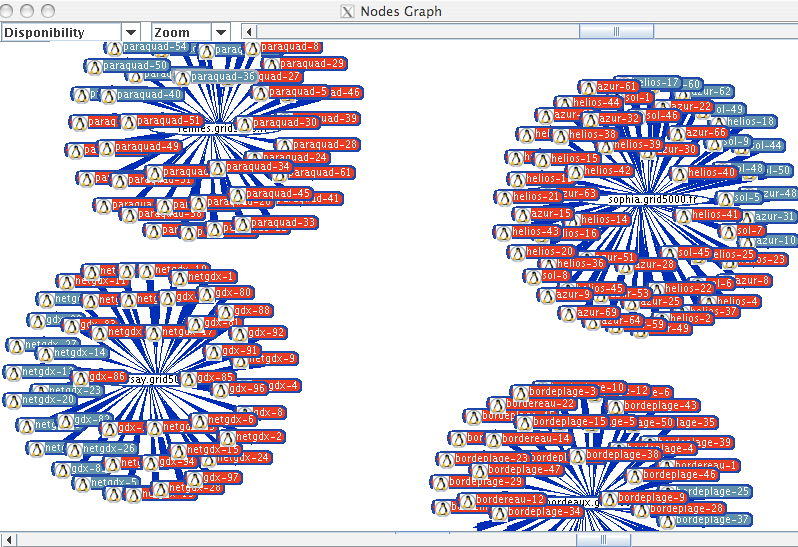
\includegraphics[width=.75\textwidth]{fig/runVisu-3.png}
\end{block}
}


\frame{
\frametitle{This Work's Objectives}

\vspace{1cm}
%\begin{exampleblock}{In one word}
%Move from a JXTA P2P infrastructure to something allowing latency-aware allocation.
%\end{exampleblock}

\begin{block}{}
	\begin{enumerate}
	\item Integrate knowledge about peer locality into a P2P-based middleware
	\item Provide simple allocation strategies to users 
      \item Assess the effectiveness of allocation strategies at a large-scale % real machines
	\end{enumerate}
\end{block}

\begin{block}{}
	... with the constraints :
	\begin{itemize}
	\item self-contained software for a simple installation,
	\item usable port range may be restricted. 
	\end{itemize}
\end{block}


}




%-------------------------------------------------------------------
%   S E C T I O N :   P2P-MPI Middleware
%-------------------------------------------------------------------
\section{P2P-MPI Middleware}

\frame{
\frametitle{What is P2P-MPI ?}
\begin{block}{P2P-MPI in a few words}
	\begin{itemize}
		\item An integrated software running in \alert{user-space},
            \item using \alert{Java} only,
		\item providing a \alert{message passing} library (MPJ),
		\item with optional transparent \alert{fault-tolerance} for applications,
		\item making the local computer join a \alert{peer-to-peer} network.
\end{itemize}
\end{block}
}

\frame{
\frametitle{Fault Tolerance: Replication Based}

\begin{itemize}
\item How much replication for each process is specified by user (option -r).
\item Guarantee : no 2 copies of a process on a same host.
\item Replication transparent to the programmer (Send $P_0 \rightarrow P_1$).
\end{itemize}

\begin{center}
\resizebox{\textwidth}{!}{\input{fig/replica.pdftex_t}}
\end{center}
}

%-------------------------------------------------------------------
\frame{
\frametitle{P2P-MPI}
\begin{overlayarea}{\textwidth}{2.2cm}


Three conceptual parts:
\begin{itemize}
\item the peer-to-peer infrastructure,
\item the middleware,
\item and the communication library.
\end{itemize}
\end{overlayarea}

\begin{center}
\resizebox{!}{.5\textheight}{\input{fig/structure.pdftex_t}}
\end{center}
}

\begin{comment}
\frame{
\frametitle{Application Start-up Scenario}

\begin{overlayarea}{\textwidth}{.75\textheight}
\only<1>{
\begin{center}
\resizebox{!}{.7\textheight}{\input{fig/scenario_1.pdftex_t}}
\end{center}
}
\only<2>{
\begin{center}
\resizebox{!}{.7\textheight}{\input{fig/scenario_2.pdftex_t}}
\end{center}
}
\only<3>{
\begin{center}
\resizebox{!}{.7\textheight}{\input{fig/scenario_3.pdftex_t}}
\end{center}
}
\only<4>{
\begin{center}
\resizebox{!}{.7\textheight}{\input{fig/scenario_4.pdftex_t}}
\end{center}
}
\only<5>{
\begin{center}
\resizebox{!}{.7\textheight}{\input{fig/scenario_5.pdftex_t}}
\end{center}
}
\only<6>{
\begin{center}
\resizebox{!}{.7\textheight}{\input{fig/scenario_6.pdftex_t}}
\end{center}
}
\only<7>{
\begin{center}
\resizebox{!}{.7\textheight}{\input{fig/scenario_7.pdftex_t}}
\end{center}
}
\only<8>{
\begin{center}
\resizebox{!}{.7\textheight}{\input{fig/scenario_8.pdftex_t}}
\end{center}
}
\only<9>{
\begin{center}
\resizebox{!}{.7\textheight}{\input{fig/scenario_9.pdftex_t}}
\end{center}
}
\only<10>{
\begin{center}
\resizebox{!}{.7\textheight}{\input{fig/scenario_10.pdftex_t}}
\end{center}
}
\only<11>{
\begin{center}
\resizebox{!}{.7\textheight}{\input{fig/scenario_11.pdftex_t}}
\end{center}
}
\only<12>{
\begin{center}
\resizebox{!}{.7\textheight}{\input{fig/scenario.pdftex_t}}
\end{center}
}
\end{overlayarea}

\begin{overlayarea}{\textwidth}{2cm}
\only<1>{ {\small \textbf{Booting up:} \texttt{mpiboot} starts \texttt{MPD, FD, FT, RS}.}}
\only<2>{ {\small \textbf{Job submission: } \texttt{p2pmpirun -n} $n$  \texttt{-r} $r$  \texttt{-a} $alloc$ \texttt{prog}.}}
\only<3>{ {\small \textbf{Requesting peers: } Application asks \texttt{MPD} to discover resources for executing $n \times r$ MPI processes.}}
\only<4>{ {\small \textbf{Discovery and Reservation: } \texttt{MPD} requests \texttt{RS} to reserve peer.}}
\only<5>{ {\small \textbf{Registering: } Local \texttt{MPD} contacts distant MPDs, give them MPI ranks, and IP, port of rank 0.}}
\only<6>{ {\small \textbf{Hand-shake: } The remote peers sends its \texttt{FD}, \texttt{FT} ports to rank 0.}}
\only<7>{ {\small \textbf{File staging: } program and data transfer via \texttt{FT}.}}
\only<8>{ {\small \textbf{Execution Notification: } \texttt{FD} notifies \texttt{MPD} to execute the transferred program.}}
\only<9>{ {\small \textbf{Remote executable lauch: } \texttt{MPD} executes the transferred program.}}
\only<10>{ {\small \textbf{Execution preamble: } spawn processes return their IP, port, rank to build the MPI communicator.}}
\only<11>{ {\small \textbf{Fault detection: } MPI processes register itself to \texttt{FD} for monitoring failure during the execution.}}
\end{overlayarea}
}

\end{comment}
%------------------------------------------------------------------
\frame{
\frametitle{Discovery and Allocation}
\begin{overlayarea}{\textwidth}{.75\textheight}
\only<1>{
\begin{center}
\resizebox{!}{.7\textheight}{\input{fig/reserv.pdftex_t}}
\end{center}
}
\only<2>{
\begin{center}
\resizebox{!}{.7\textheight}{\input{fig/reserv_1.pdftex_t}}
\end{center}
}
\only<3>{
\begin{center}
\resizebox{!}{.7\textheight}{\input{fig/reserv_2.pdftex_t}}
\end{center}
}
\only<4>{
\begin{center}
\resizebox{!}{.7\textheight}{\input{fig/reserv_3.pdftex_t}}
\end{center}
}
\only<5>{
\begin{center}
\resizebox{!}{.7\textheight}{\input{fig/reserv_4.pdftex_t}}
\end{center}
}
\only<6>{
\begin{center}
\resizebox{!}{.7\textheight}{\input{fig/reserv_5.pdftex_t}}
\end{center}
}
\only<7>{
\begin{center}
\resizebox{!}{.7\textheight}{\input{fig/reserv_6-0.pdftex_t}}
\end{center}
}
\only<8>{
\begin{center}
\resizebox{!}{.7\textheight}{\input{fig/reserv_6.pdftex_t}}
\end{center}
}
\only<9>{
\begin{center}
\resizebox{!}{.7\textheight}{\input{fig/reserv_7.pdftex_t}}
\end{center}
}
\end{overlayarea}

\begin{overlayarea}{\textwidth}{2cm}
\only<1>{ \framebox{{\small Each peer maintains \alert{peer list} sorted by ping time (cache of supernode's list).}}}
\only<2>{ {\small \textbf{Requesting peers: } \texttt{p2pmpirun -n} $n$  \texttt{-r} $r$  \texttt{-a} $alloc$ \texttt{prog} $\Rightarrow$ we need at most $n \times r$ peers. Run discovery.}}

\only<3>{ {\small \textbf{Booking: } \texttt{MPD} requests \texttt{RS} a reservation for the first $(n \times r) + (3log_2(n \times r))$ (overbooking) peers of its sorted list.}}

\only<4>{ {\small \textbf{RS-RS brokering: } \texttt{RS} generates a \emph{unique hash key} then send it to remote \texttt{RS} to reserve peer.}}
\only<5>{ {\small \textbf{Reservation result: } \texttt{RS} returns OK and how many processes it can accept (capacity) or NOK.}}
\only<6>{ {\small \textbf{RS-MPD reponse: } local \texttt{RS} gathers the answer from remote {RS}, forms \emph{rlist}, and then pass it to local \texttt{MPD}.}}
\only<7>{ {\small \textbf{Node assignment: } MPD computes node ranks depending on \alert{allocation strategy}.}}
\only<8>{ {\small \textbf{Allocation: } \texttt{MPD} allocates node and give its rank.}}
\only<9>{ {\small \textbf{Verify reservation: } \texttt{MPD} checks with \texttt{RS}, if the application has a reservaton before execution using the hash key.}}

\end{overlayarea}
}
%------------------------------------------------------------------
\begin{comment}
\frame{
\frametitle{Allocation feasibility}
%\begin{block}{}
A number of RS have Let :\\
\begin{itemize}
\item \alert{$n$} be the number of MPI logical processes (from \texttt{-n} $n$).
\item \alert{$r$} be the number of copied processes for each logical process (from \texttt{-r} $r$).
\item \alert{$P_{i}$} be the number of processes allow to execute on node $i$ by single application.
\item \alert{$rlist$} be the list of reserved nodes (overbooking).
\item \alert{$slist$} be the list of selected nodes chosen to map the application processes.


\item $slist = rlist[1, \ldots, \min( |rlist|, n \times r)]$.
\end{itemize}
%\end{block}
}
\end{comment}

\begin{comment}
\begin{overlayarea}{\textwidth}{1cm}
\only<1>{
(1) check feasibility.
}
\only<2>{
(2) process allocation depending on strategy.
}
\end{overlayarea}
\end{comment}

\frame{
\frametitle{Problematics: Host Allocation}
2 steps : 
\begin{enumerate}
\item<1> check feasibility.
\item<2> process allocation depending on strategy.
\end{enumerate}

\textbf{Example :} \texttt{p2pmpirun -n 2 -r 2 prog}\\
\textbf{System :} $H_1$ quad-core, $H_2$ and $H_3$ dual-core.

\vspace{1cm}
\begin{overlayarea}{\textwidth}{2cm}
\only<1>{
\begin{center}
\resizebox{0.75\textwidth}{!}{\input{fig/allo_feasibility_1.pdftex_t}}
\end{center}
}
\only<2>{
\begin{center}
\resizebox{0.75\textwidth}{!}{\input{fig/allo_feasibility_2.pdftex_t}}
\end{center}
}
\end{overlayarea}
}

\frame{
\frametitle{Allocation feasibility}
%\begin{block}{}
\alert{$slist$}: selected peers with a reservation ($ \leq  n \times r)$.\\
\alert{$P_{i}$}: number of processes offered by peer $i$ for a given application.\\
\vspace{.5cm}

Allocation is possible if the two following conditions are met:
\begin{enumerate}

\item<+-> $ |slist| \ge r$ ~~\textit{(No two replicas on a same host)}
\begin{columns}[c]
\column{.5\textwidth}
\begin{center}
\resizebox{.5\textwidth}{!}{\input{fig/no_alloc1.pdftex_t}}
\end{center}
\column{.5\textwidth}
\begin{exampleblock}{\texttt{p2pmpirun -n 2 -r 2}}
$|slist| = 1 < r = 2$
\end{exampleblock}
\end{columns}

\item<+-> $\sum_{i=0}^{|slist|} c_{i} \ge n \times r$, where $c_{i} = \min (P_{i}, n)$.  \textit{(Enough ``slots'')}
\begin{columns}[c]
\column{.5\textwidth}
\begin{center}
\resizebox{.75\textwidth}{!}{\input{fig/no_alloc2.pdftex_t}}
\end{center}
\column{.5\textwidth}
\begin{exampleblock}{\texttt{p2pmpirun -n 2 -r 2}}
$|slist| = 2 \ge r = 2$ \alert{$\surd$}\\
$c_{0} = \min (4, 2) = 2$\\
$c_{1} = \min (1, 2) = 1$\\
$\sum_{i=0}^{1} c_{i} = 3 <  n \times r = 4$
\end{exampleblock}
\end{columns}


\end{enumerate}
}

%------------------------------------------------------------------
\begin{comment}
\frame{
\frametitle{Host allocation constraints}
\begin{block}{}
Once $slist$ has been extracted, and before the MPI ranks distribution can take place,
the MPD must decide whether the allocation is feasible.
\end{block}
\vspace{0.3cm}
It is feasible if the two following conditions are met:
\begin{enumerate}
\item $ |slist| \ge r$


\item $\sum_{i=0}^{|slist|} c_{i} \ge n \times r$, where $c_{i} = \min (P_{i}, n)$.
\end{enumerate}
}
\end{comment}

%------------------------------------------------------------------
\begin{comment}
\frame{
\frametitle{Host allocation criteria}
\begin{block}{}
There are today many multicore CPUs and we should
favor the allocation of processes on all cores of a CPU if we strictly
follow the locality principle.\\

However it might be more important for the application to access more
memory on the whole, which is in contradiction to the allocation
strategy that chooses all cores on each resource as they share the same memory.
\end{block}

\pause
In our context, an allocation strategy must meet two criteria :
\begin{enumerate}
\item<+->
It must assign the $n{\times}r$ processes to the $|slist|$  reserved hosts
in a sensible and understandable way regarding the user's concerns.
\item<+->
In case some processes are replicated, the rank assigned to mapped processes must
guarantee that no two copies of a process are on the same processor.
\end{enumerate}
}
\end{comment}
%------------------------------------------------------------------
\frame{
\frametitle{Host Allocation Strategies}
Two simple host allocation strategies:
\pause
\vspace{0.2cm}
\begin{enumerate}
\item<+-> \textbf{Spread} round-robin \alert{host-wise}: less processes using a memory bank,
more out-of-host communications.

\begin{overlayarea}{\textwidth}{2cm}
\only<2,3>{
\begin{center}
\resizebox{.65\textwidth}{!}{\input{fig/spread_alloc.pdftex_t}}
\end{center}
}
\end{overlayarea}
 
\item<+-> \textbf{Concentrate} round-robin \alert{core-wise}: more intra-host communications,
less memory available per process % assuming all cores share a same memory bank
and more memory access contention.
\begin{overlayarea}{\textwidth}{2cm}
\only<3>{
\begin{center}
\resizebox{.65\textwidth}{!}{\input{fig/concentrate_alloc.pdftex_t}}
\end{center}
}
\end{overlayarea}
\end{enumerate}
}

%------------------------------------------------------------------
\frame{
\frametitle{Host allocation strategies}
\begin{exampleblock}{Spread algorithm}
\begin{small}
\begin{algorithm}[H]
\dontprintsemicolon
        d := 0\;
        $\forall_{i}, {u_i}$ := 0\;
        cont:= TRUE\;
        \While{cont}{
                i := 0\;
                \While{$(i < |slist|)$ AND cont}{
                        \If{$(u_i < c_i)$}{
                               $u_i := u_i + 1$\;
                               d := d + 1\;
                        }
                        \If{$(d = n \times r)$}{
                                cont := FALSE\;
                        }
                        i := i + 1\;
                }
        }
\end{algorithm}
\end{small}
\end{exampleblock}
}

%------------------------------------------------------------------
\frame{
\frametitle{Host allocation strategies}
\begin{exampleblock}{Concentrate algorithm}
\begin{small}
\begin{algorithm}[H]
\dontprintsemicolon
        d := 0\;
        $\forall_{i}, {u_i}$ := 0\;
        cont := TRUE\;
        \While{cont}{
                i := 0\;
                \While{$(i < |slist|)$ AND cont}{
                        $u_i := min(c_i, (n \times r) - d)$\;
                        $d := d + u_i$\;
                        \If{$(d = n \times r)$}{
                                cont := FALSE\;
                        }
                        i := i + 1\;
                }
        }
\end{algorithm}
\end{small}
\end{exampleblock}
}

\frame{
\frametitle{Host allocation strategies}
\begin{exampleblock}{Rank assigning algorithm }
\begin{small}
\begin{algorithm}[H]
\dontprintsemicolon
        rank := 0\;
        \For{host $i$ in $slist$}{
                \If{$u_i = 0$}{
                        cancel reservation on host $i$\;
                }
                l := 0\;
                \While{$l < u_i$}{
                        assign rank $rank$ to host $i$\;
                        rank := rank + 1\;
                        l := l + 1\;
                        \If{$rank \geq n$}{
                                rank := 0\;
                        }
                }
        }
\end{algorithm}
\end{small}
\end{exampleblock}
}

\section{Allocation Experiment}
%--------------------------------------------------------------------------
% GRID 5000
%--------------------------------------------------------------------------
\frame{
\frametitle{GRID'5000}
\begin{center}
\resizebox{.6\textwidth}{.55\textheight}{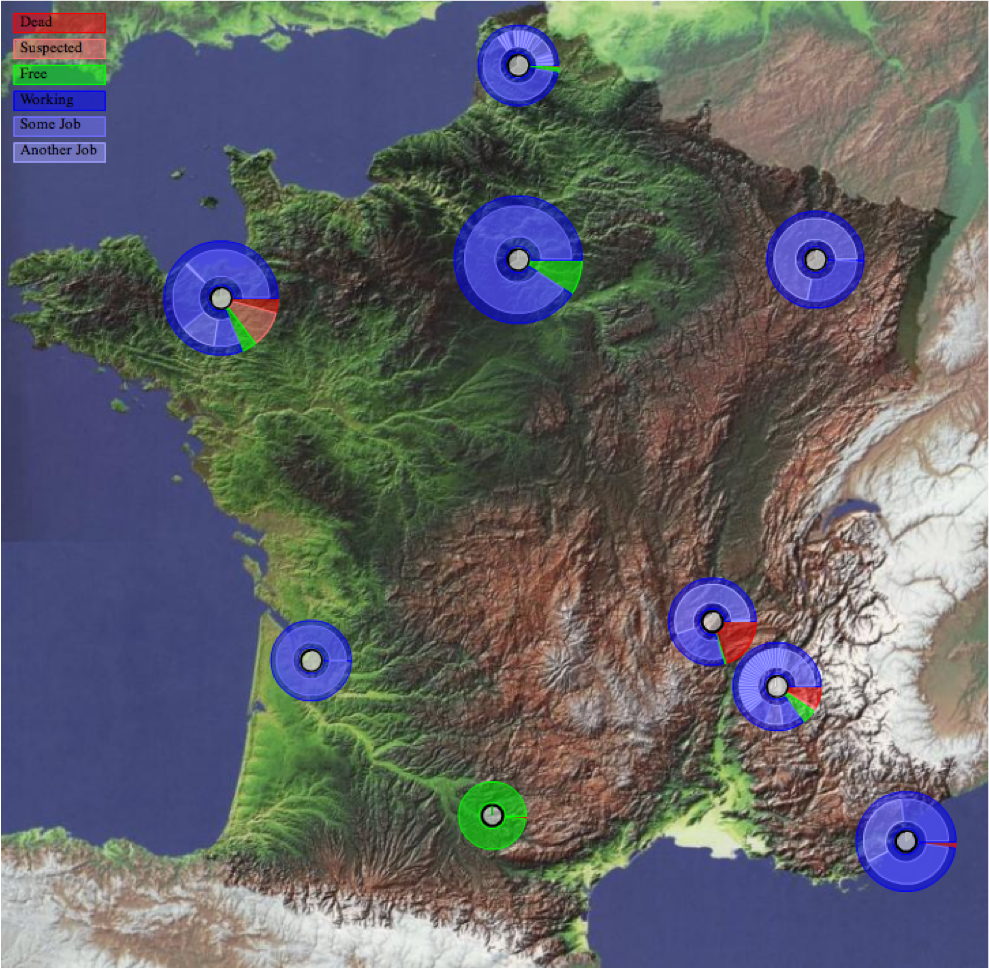
\includegraphics[width=.75\textwidth]{fig/g5k.png}}
\end{center}
\begin{block}{Grid'5000}
\begin{scriptsize}
\begin{itemize}
\item A set of clusters (Opteron, Xeon, Itanium),
\item Currently : $\approx$ 4400 cores, in more than 1500 dual or quad-core hosts,
\item 9 geographical sites in France ($\approx$ 1000 kms),
\item Interconnected by backbone links (RENATER) offering 1 or 10 Gbps.
\end{itemize}
\end{scriptsize}
\end{block}
}

\begin{comment}
\frame{
\frametitle{Grid'5000: network characteristics}
\begin{columns}
\begin{column}{9cm}
\textcolor{blue}{Grid'5000} $\rightarrow$ since nov 2005 : \underline{Renater-4}
\pause
\begin{itemize}
\item partly based on a DWDM (Dense Wave Division Multiplexing) infrastructure:
\begin{itemize}
\item infrastructure exclusively used (today) by 3 projects (G5K, LHC, DEISA),
\item enables a \em{lightpath} between 2 sites.
\end{itemize}
\item aug 2006: 6 sites have access to the DWDM infrastructure:
\begin{itemize}
\item 3 sites at 10 Gbps VLAN (Nancy, Rennes, Nice),
\item 3 sites at 1 Gbps (Grenoble,Lille,Toulouse),
\item other sites were linked via Ethernet Over MPLS (1Gpbs).
\end{itemize}
\item moving toward 10\,Gbit/s connections for all sites. Status:
\scriptsize{\url{https://www.grid5000.fr/mediawiki/index.php/Network\_interlink\#Renater4}}

%% au 18 mars 2007, tous les sites sont connectes au DWDM (interface dark fiber)
%% sauf Bordeaux et Orsay.

\end{itemize}
\end{column}

\begin{column}{3cm}
\includegraphics[width=\linewidth]{fig/renater4.pdf}
\end{column}
\end{columns}
}


\frame{
\frametitle{Renater-4 map}

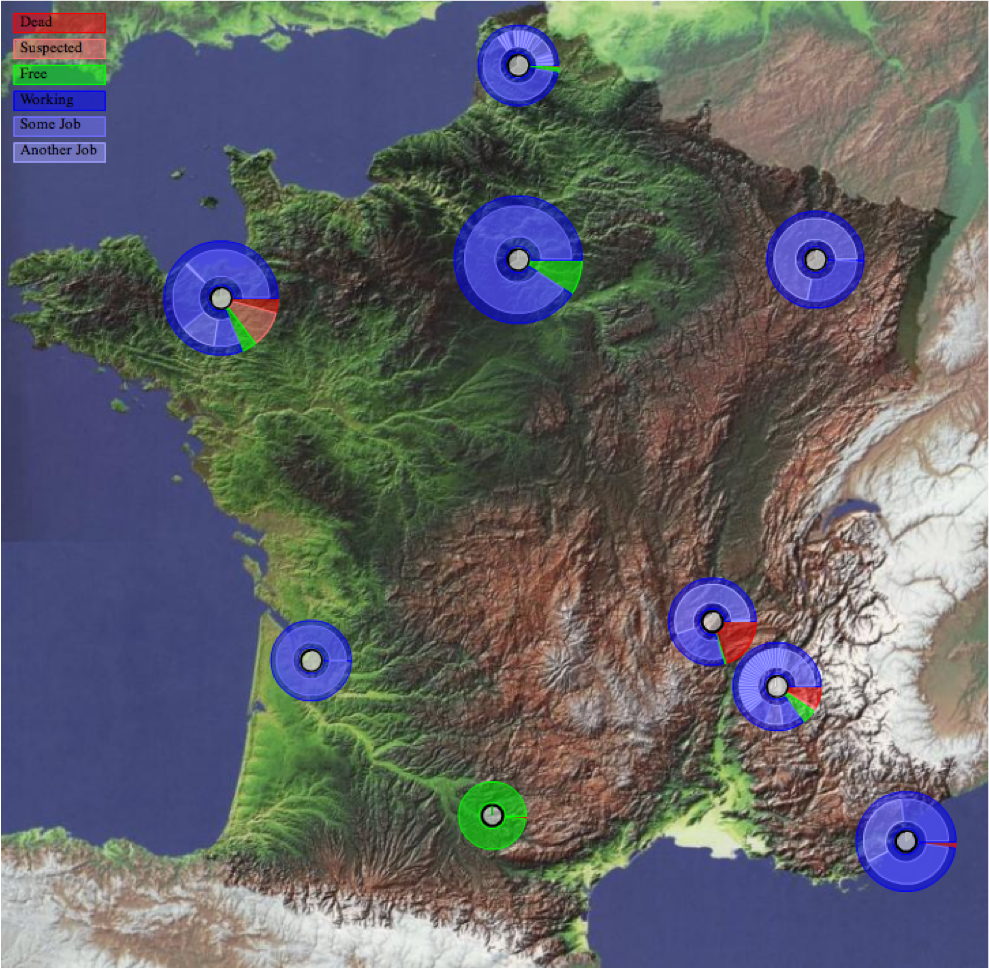
\includegraphics[width=.75\textwidth]{fig/g5k.png}
%\includegraphics[width=.75\textwidth]{fig/renater4.pdf}

}
\end{comment}

\begin{comment}
\frame{
\frametitle{Network latencies}

\begin{center}
\begin{table}[t]
\begin{center}
\resizebox{\textwidth}{!}{
%\rowcolors[]{1}{blue!20}{blue!10}
\begin{tabular}{|l|cccccc|}
\hline
& strasbourg & orsay & rennes & toulouse & nice & lyon \\
\hline
strasbourg & -- & 5.06/0.03 &7.64/0.03 & 9.74/0.03 & 11.92/0.02 & 6.49/0.02 \\
orsay & 3.28/0.03 & -- & 3.54/0.03 & 5.44/0.03 & 9.07/0.02 & 2.49/0.02 \\
rennes & 7.80/0.02 & 5.39/0.02 & -- & 6.36/0.01 & 9.14/0.01 & 8.17/0.01 \\
toulouse & 8.13/0.02 & 5.34/0.02 & 4.40/0.01 & -- & 2.85/0.01 & 2.53/0.01 \\
nice & 12.23/0.02 & 10.95/ & 9.11/0.01 & 4.77/0.01 & -- & 5.78/0.01 \\
lyon & 6.51/0.02 & 5.25/0.02 & 7.93/0.02 & 4.21/0.01 & 5.48/0.02 & -- \\
\hline
\end{tabular}
}
\end{center}
\end{table}
\medskip
{\small Renater\,4 latencies
{\scriptsize (latency/standard deviation in ms)}}.
\end{center}
source: Renater sensors\\
\scriptsize{\url{http://pasillo.renater.fr/metrologie/get\_qosmetrics\_results.php}}
}
\end{comment}
%------------------------------------------------------------------------------------------


\frame{
\frametitle{Experiments}

Experiment Setup :\\

\begin{table}[H]
\begin{center}
\resizebox{1\textwidth}{!}{
      \begin{tabular}{|l|l|l|l|l|l|}
      \hline
      \multicolumn{1}{|l|}{Environment type} &
      \multicolumn{5}{|l|}{Grid5000 -- clusters as detailed below.}\\
      \hline
      Site    & Cluster name  & CPU & \#Nodes   & \#CPUs   & \#Cores\\
      \hline
      Nancy&  grelon & Intel Xeon 5110  & 60 & 120 & 240\\
      Lyon&  capricorn & AMD Opteron 246 & 50 & 100  & 100\\
      Rennes& paravent & AMD Opteron 246  & 90 & 180 & 180\\
      Bordeaux& bordereau & AMD Opteron 2218 & 60 & 120 & 240\\
      Grenoble& idpot & Intel Xeon IA32 & 8 & 16 &16\\
      Grenoble&idcalc& Intel Itanium 2 & 12 & 24 & 48\\
      Sophia-Antipolis& azur & AMD Opteron 246 & 32&64&64\\
      Sophia-Antipolis& sol & AMD Opteron 2218 & 38& 76& 152\\
      \hline
      \multicolumn{1}{|l|}{Operating System} &
      \multicolumn{5}{|l|}{Linux 2.6.18 or close}\\
      \hline
      \multicolumn{1}{|l|}{Software} &
      \multicolumn{5}{|l|}{jdk1.6.0\_04, JXTA-J2SE 2.3, p2pmpi-0.28.0}\\
      \hline
      \end{tabular}
}
\end{center}
\end{table}
}

\frame{
\frametitle{ICMP}
ICMP Ping :
\begin{table}[H]
\begin{center}
  \begin{tabular}{|l|l|}
      \hline
      Site    & RTT(ms)\\
      \hline
      Lyon& 10.5\\
      Rennes& 11.6\\
      Bordeaux& 12.6\\
      Grenoble& 13.2\\
      Sophia-Antipolis&17.1\\
      \hline
      \end{tabular}
\end{center}
\end{table}

\begin{exampleblock}{Question}
How close are we from ICMP measurements ?
\end{exampleblock}

}

\frame{
\frametitle{Experiment: Concentrate Allocation Strategy}
{\footnotesize \textbf{Job submitter :} Nancy site.}\\
{\footnotesize \textbf{Network Lantency (ICMP from Nancy):}}\\
{\footnotesize Nancy $<$ Lyon $<$ Rennes $<$ Bordeaux $<$ Grenoble $<$ Sophia.}
\begin{columns}[c]
\column{.5\textwidth}
\begin{figure}[H]
\includegraphics[width=\textwidth]{fig/gather_result_host_allocated.pdf}\\
\vspace{-0.2cm}
{\footnotesize (a) Allocated hosts.}
\end{figure}

\column{.5\textwidth}
\begin{figure}[H]
\includegraphics[width=\textwidth]{fig/gather_result_proc_allocated.pdf}\\
\vspace{-0.2cm}
{\footnotesize (b) Allocated cores.}
\end{figure}
\end{columns}
\vspace{0.25cm}
\begin{itemize}
\item {\footnotesize Nancy has 240 cores.}
\item {\footnotesize Beyond 240 processes, Rennes, Bordeaux, Lyon hosts are chosen.}
\end{itemize}
}



\frame{
\frametitle{Experiment: Spread Allocation Strategy}
{\footnotesize \textbf{Job submitter :} Nancy site.}\\
{\footnotesize \textbf{Network Lantency (ICMP from Nancy):}}\\
{\footnotesize Nancy $<$ Lyon $<$ Rennes $<$ Bordeaux $<$ Grenoble $<$ Sophia.}
\begin{columns}[c]
\column{.5\textwidth}

\begin{figure}[H]
\includegraphics[width=\textwidth]{fig/scatter_result_host_allocated.pdf}\\
\vspace{-0.2cm}
{\footnotesize (a) Allocated hosts.}
\end{figure}

\column{.5\textwidth}
\begin{figure}[H]
\includegraphics[width=\textwidth]{fig/scatter_result_proc_allocated.pdf}\\
\vspace{-0.2cm}
{\footnotesize (b) Allocated cores.}
\end{figure}
\end{columns}
\vspace{0.25cm}
\begin{itemize}
\item {\footnotesize Sophia hosts are chosen when $>$ 280 processes requested.}
\item {\footnotesize The allocation distributes again to Nancy when $>$ 380 processes.}
\end{itemize}

}

\frame{
\frametitle{Application Performances}
\begin{columns}[c]
\column{.5\textwidth}
\begin{figure}[H]
\includegraphics[width=\textwidth]{fig/ep_result.pdf}\\
{\small (a) EP benchmark.}
\end{figure}

\column{.5\textwidth}
\begin{figure}[H]
\includegraphics[width=\textwidth]{fig/is_result.pdf}\\
{\small (b) IS benchmark.}
\end{figure}

\end{columns}
}


%-----------------------------------------------------
% SECTION : Conclusion
%-----------------------------------------------------
\section{Conclusion and Future work}
\frame{
\frametitle{Conclusion and Future Work}
\begin{itemize}
\item P2P-MPI is a self-contained piece of software (no helper service)
offering a fault-tolerant MPJ implementation.
\item Now integrates information about peers network proximity.  
\item Provides simple and understandable strategies to the user.
\item Experiments show allocation results close to those expected. 
\item Improve the network performance measurement. 
\item Integrate other selection criteria in strategies.
\item Allow users to describe their own strategy.
\end{itemize}
}



\frame{
\frametitle{Thank you}
\begin{center}
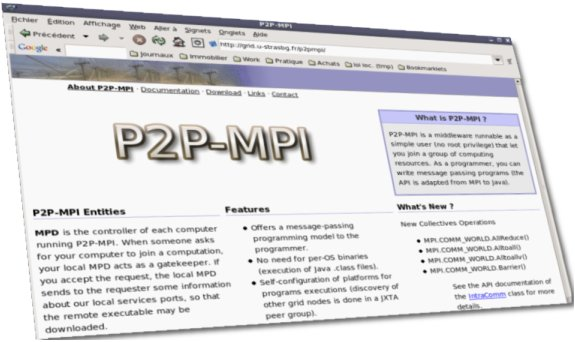
\includegraphics[height=.6\textheight]{fig/website.jpg}\\

\url{http://www.p2pmpi.org}
\end{center}


}




\end{document}
